\chapter{mainline}
\label{sec:listing}
\lstset{style=6502Style}
\lhead[tempest]{}

Tempest's 'mainline' is a short routine that runs the entirety of the game from a handful of lines
of assembly code. Beneath lies an iceberg of strange machinery but at its core the game consists of
running these 15 or so lines many hundreds of times per second:

\begin{lstlisting}
;INPUT:         POWER ON RESET PREPARATION
;OUTPUT:        NONE

MAINLN: JSR INISOU              ;INITIALIZE SOUNDS
        LDA I,CNEWGA
        STA QSTATE
        BEGIN                   ;MAINLOOP
        BEGIN                   ;LOOP UNTIL CURRENT FRAME HAS BEEN UP X MS.
        LDA FRTIMR
        CMP I,9
        CSEND
        LDA I,0                 ;RESTART FRAME TIMER
        STA FRTIMR
        JSR EXSTAT              ;EXECUTE APPROPRIATE GAME STATE
        JSR NONSTA              ;EXECUTE NON-STATE DEPENDENT CODE
        JSR DISPLA              ;EXECUTE CODE TO DISPLAY NEW SCREEN
        CLC
        CSEND                   ;LOOP ALWAYS
\end{lstlisting}

The game's framerate is controlled by this tight little loop. As soon as \icode{FRTIMR} reaches 9 a frame
of the game is executed:
\begin{lstlisting}
        LDA FRTIMR
        CMP I,9
        CSEND
\end{lstlisting}

\begin{figure}[H]
  \centering
  \frame{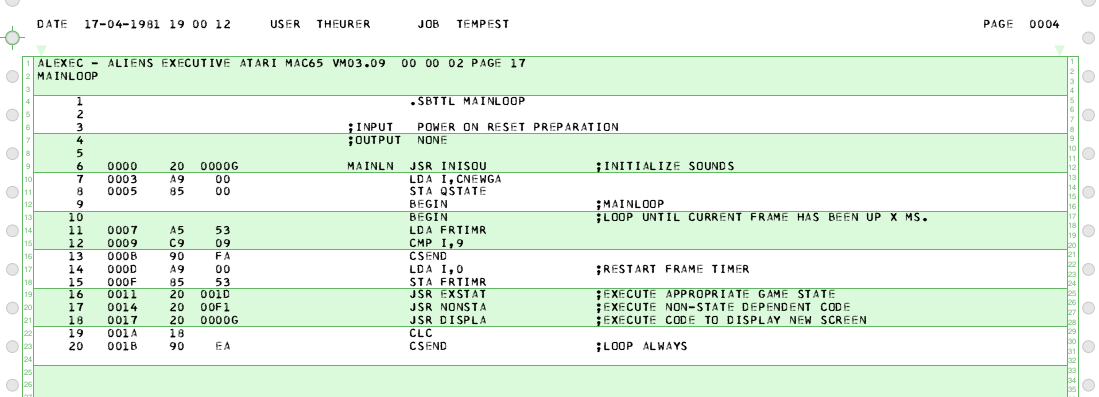
\includegraphics[width=13cm]{src/build/mainline.png}}%
  \caption{The \icode{MAINLN} routine in an assembly listing.}
\end{figure}
\begin{figure}[H]
  \centering
  \frame{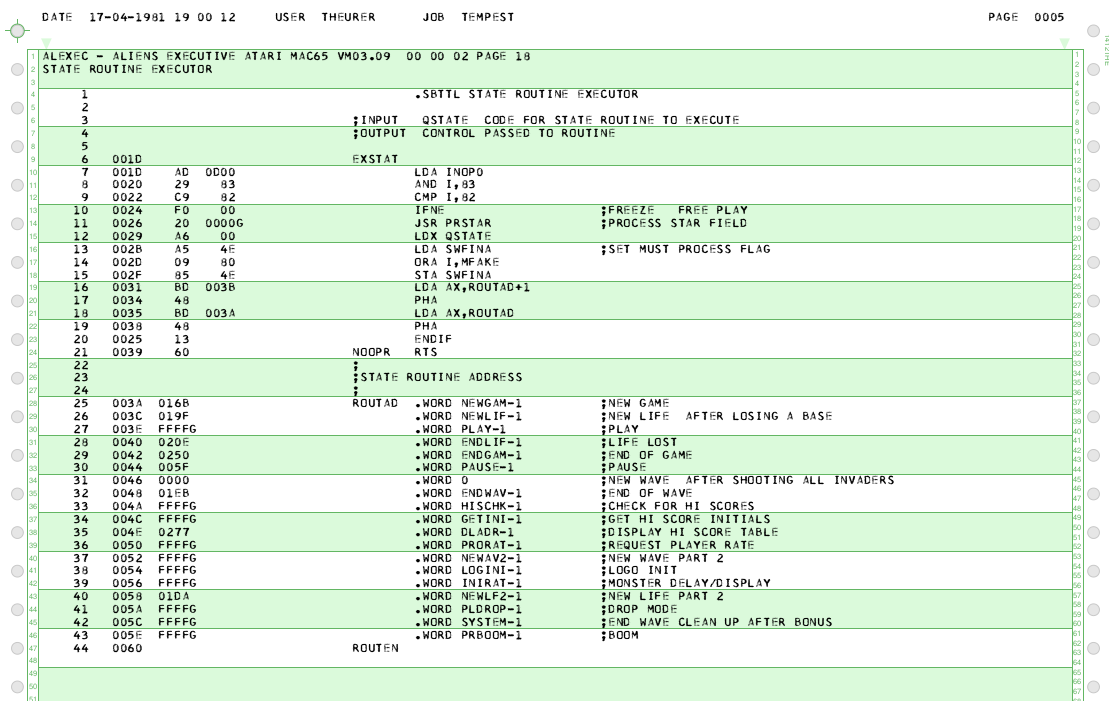
\includegraphics[width=13cm]{src/build/exstat.png}}%
  \caption{The \icode{EXSTAT} and \icode{ROUTEAD} routines in an assembly listing.}
\end{figure}
\clearpage

Then it is reset to zero:
\begin{lstlisting}
        LDA I,0                 ;RESTART FRAME TIMER
        STA FRTIMR
\end{lstlisting}
Increasing the value from \icode{9} to \icode{0F} (15) will slow the game down appreciably, while increasing
it to \icode{1F} (31) will bring it to an unplayable crawl. Lowering it to \icode{0} or \icode{1} does make the game slightly
faster, but not noticeably and it is still playable.

\begin{definition}[cursor says\index{cursor says}]
\setlength{\intextsep}{0pt}%
\setlength{\columnsep}{3pt}%
\begin{wrapfigure}{l}{0.12\textwidth}

\includegraphics[width=\linewidth]{src/callout/claw_t.png} 
\end{wrapfigure}
\small
\textcolor{white}{
  But what increments \icode{FRTIMR} you ask? The answer is a piece of code in what is known
  as an 'interrupt handler'. This runs separately from the main loop and is invoked by the CPU up to 60
  times a second.
}
\end{definition}

Once we've decided to execute a frame we are down to just three lines orchestrating the entirety of the game:

\begin{lstlisting}
        JSR EXSTAT              ;EXECUTE APPROPRIATE GAME STATE
        JSR NONSTA              ;EXECUTE NON-STATE DEPENDENT CODE
        JSR DISPLA              ;EXECUTE CODE TO DISPLAY NEW SCREEN
\end{lstlisting}

The first routine we call is \icode{EXSTAT}. It always updates the starfield (\icode{PRSTAR}) but what it
does next is dependent on the value contained in \icode{QSTATE}. Take a brief look at the routine to see if
you can identify how it uses \icode{QSTATE}:
\begin{lstlisting}
;INPUT:         QSTATE: CODE FOR STATE ROUTINE TO EXECUTE
;OUTPUT:        CONTROL PASSED TO ROUTINE

EXSTAT:
        LDA INOP0
        AND I,83
        CMP I,82
        IFNE                    ;FREEZE & FREE PLAY?
        JSR PRSTAR              ;PROCESS STAR FIELD
        LDX QSTATE
        LDA SWFINA              ;SET MUST PROCESS FLAG
        ORA I,MFAKE
        STA SWFINA
        LDA AX,ROUTAD+1
        PHA
        LDA AX,ROUTAD
        PHA
        ENDIF
NOOPR:  RTS
\end{lstlisting}

The answer is in these lines:
\begin{lstlisting}
        LDX QSTATE
        ..
        LDA AX,ROUTAD+1
        PHA
        LDA AX,ROUTAD
        PHA
\end{lstlisting}

The value in \icode{QSTATE} is loaded to the \icode{X} register. This is then used an index to retrieve the two-byte address
stored in the \icode{X}th - 1 index of the \icode{ROUTAD} table: 
\begin{lstlisting}
;
;STATE ROUTINE ADDRESS
;
ROUTAD: .WORD NEWGAM-1          ;NEW GAME
        .WORD NEWLIF-1          ;NEW LIFE (AFTER LOSING A BASE)
        .WORD PLAY-1            ;PLAY
        .WORD ENDLIF-1          ;LIFE LOST
        .WORD ENDGAM-1          ;END OF GAME
        .WORD PAUSE-1           ;PAUSE
        .WORD 0                 ;NEW WAVE (AFTER SHOOTING ALL INVADERS)
        .WORD ENDWAV-1          ;END OF WAVE
        .WORD HISCHK-1          ;CHECK FOR HI SCORES
        .WORD GETINI-1          ;GET HI SCORE INITIALS
        .WORD DLADR-1           ;DISPLAY HI SCORE TABLE
        .WORD PRORAT-1          ;REQUEST PLAYER RATE
        .WORD NEWAV2-1          ;NEW WAVE PART 2
        .WORD LOGINI-1          ;LOGO INIT
        .WORD INIRAT-1          ;MONSTER DELAY/DISPLAY
        .WORD NEWLF2-1          ;NEW LIFE PART 2
        .WORD PLDROP-1          ;DROP MODE
        .WORD SYSTEM-1          ;END WAVE CLEAN UP AFTER BONUS
        .WORD PRBOOM-1          ;BOOM
\end{lstlisting}

Pushing each of the two bytes to the stack (using \icode{PHA}) means that whatever is at the address of those two bytes will
be executed next. For example, if the value in \icode{QSTATE} is \icode{0} it will retrieve the address of \icode{NEWGAM-1}: which is
\icode{016B}, made up of \icode{6B} which it retrieves first, and \icode{01} which it retrieves second. When both of these bytes
are pushed to the stack they are treated as an address for execution: the result is that the \icode{EXTSTAT} routine will execute
\icode{NEWGAM} once it exits, beginning a new game. 

So depending on the current state of the game, Tempest will populate \icode{QSTATE} with the index for the function it needs
to call next. To give a flavour of what \icode{NEWGAM} looks like we've listed it below. As expected it mainly consists of 
accounting operations such as clearing the score, assigning the number of lives and so on. 

\begin{lstlisting}
NEWGAM: JSR INICHK              ;INITIALIZE LANGUAGE PTRS, OPTIONS
        JSR INIDSP              ;INITIALIZE DISPLAY
        LDA QSTATUS
        IFMI                    ;ATTRACT?
        JSR CLRSCO              ;NO. CLEAR SCORES
        ENDIF
        LDA I,0
        STA LIVES2              ;ONE PLAYER GAME (DEFAULT: PLAYER 2 DEAD)
        LDX NUMPLA              ;GIVE EACH PLAYER "NEW GAME" EQUIP
        STX PLAYUP
        BEGIN                   ;LOOP FOR EACH PLAYER IN GAME (1 OR 2)
        LDX PLAYUP
        LDA LVSGAM              ;GET # LIVES
        STA AX,LIVES1           ;INITIAL # OF LIVES (GUNS)
        LDA I,-1
        STA AX,WAVEN1           ;FORCE REQUEST RATE STATE
        DEC PLAYUP
        MIEND                   ;ENDLOOP AFTER ALL PLAYERS PROCESSED
        LDA I,0
        STA NEWPLA              ;START GAME WITH 1ST PLAYER UP.
        STA PLAGRO              ;DEACTIVATE STAR FIELD
        LDA NUMPLA              ;INDUCE "PLAY PLAYER 1" MESSAGE
        STA PLAYUP              ;IF 2 PLAYER GAME.
        JMP INIRA0              ;INITIALIZE FOR PLAYER RATE REQUEST
\end{lstlisting}

You will notice at the end that we jump to a routine called \icode{INIRA0}. This continues the accounting set-up for a new
game but it also does something important, which is update \icode{QSTATE} to direct the flow the next time it passes through
\icode{MAINLN} to a different function. In this case, it loads \icode{16} to \icode{QSTATE}, which will direct us to the routine
\icode{PRORAT} at the next iteration:
\begin{lstlisting}
        LDA I,CREQRAT           ;GO TO REQUEST
        STA QSTATE              ;RATE STATE
\end{lstlisting}

Another way of describing what we have here is a 'state machine'. As the state of the system changes, \icode{EXSTAT} will execute
a different routine, appropriate to the current state of the game. The one executed most often is the third one listed in our
\icode{ROUTEAD} table. This is called \icode{PLAY} and its contents, as well as its name, are almost self-explanatory:

\begin{lstlisting}
PLAY:
        JSR MOVCUR              ;MOVE CURSOR AROUND
        JSR FIREPC              ;FIRE PLAYER CHARGE
        JSR PROSUZ              ;PROCESS SUPER ZAP
        JSR MOVNYM              ;MOVE NYMPHS
        JSR MOVINV              ;MOVE INVADERS
        JSR MOVCHA              ;MOVE CHARGES
        JSR FIREIC              ;FIRE INVADER CHARGE
        JSR COLLIS              ;COLLISION DETECT
        JSR PROEXP              ;EXPLOSIONS
        JMP ANALYZ              ;ANALYZE PLAYER STATUS
\end{lstlisting}

Here every element of the game is updated and manipulated in some way. It is not surprising that somewhere in the heart of a
game's runtime the logic should ultimately settle on a list of items that need to be checked, one after the other. One important
thing to note here is that we're not updating how any of the game elements are displayed. We are just updating their state, which
we store separately from the details of how they are displayed. We will use this updated state to determine their display in a moment,
but for now we are just updating our record of their position and condition. The second thing to note is that the order in which
these operations are performed is not arbitrary. First we update the player and any bullets the player has fired. Then we move the
enemies and any bullets they have fired. Now we can check if the player has collided with any of the enemies. If there has been a
collision between any two objects we process an explosion and finally update the player's state to determine, for example, if they are dead. The purpose
of this order is to ensure that information about the player and its enemies are updated before we detect to attempt any collisions.

A lot has happened underneath the single line..

\begin{lstlisting}
        JSR EXSTAT              ;EXECUTE APPROPRIATE GAME STATE
\end{lstlisting}

.. however now that we have all the properties of the game in its current frame we can move on to updating how they are displayed:
\begin{lstlisting}
        JSR DISPLA              ;EXECUTE CODE TO DISPLAY NEW SCREEN
\end{lstlisting}

Again this will in most cases boil down to updating all of the elements one by one. Unlike when we were concerned with updating
state, the order in which we do things is not particularly important here. The \icode{DISPLA} routine wants to build a list of lines
to paint on the screen so it will compute the lines for each type of object currently displayed in a more or less abitrary sequence
determined by the programmer. Notice that in the sequence below the display of each type of object follows a fixed pattern:

\begin{lstlisting}
                                ;DISPLAY CURSOR (PLAYER)
        LDA I,BCCURS
        JSR SBCLOG
        JSR DSPCUR
        LDA I,BCCURS
        JSR SBCSWI
                                ;DISPLAY CHARGES
        LDA I,BCSHOT
        JSR SBCLOG
        JSR DSPCHG
        LDA I,BCSHOT
        JSR SBCSWI
                                ;DISPLAY INVADERS
        LDA I,BCINVA
        JSR SBCLOG
        JSR DSPINV
        LDA I,BCINVA
        JSR SBCSWI
                                ;DISPLAY EXPLOSIONS
        LDA I,BCEXPL
        JSR SBCLOG
        JSR DSPEXP
        LDA I,BCEXPL
        JSR SBCSWI
                                ;DISPLAY NYMPHS
        LDA I,BCNYMP
        JSR SBCLOG
        JSR DSPNYM
        LDA I,BCNYMP
        JSR SBCSWI
                                ;DISPLAY INFORMATION (SCORES, MSGS, ETC.)
        LDA I,BCINFO
        JSR SBCLOG
        JSR INFO
        LDA I,BCINFO
        JSR SBCSWI
        ..
        JSR DSPWEL              ;DISPLAY WELL

        LDA I,BCENEL            ;DISPLAY ENEMY LINES
        JSR SBCLOG
        JSR DSPENL
        LDA I,BCENEL
        JSR SBCSWI

        LDA I,BCSTAR            ;DISPLAY STAR FIELD
        JSR SBCLOG
        JSR DSTARF
        LDA I,BCSTAR
        JSR SBCSWI
\end{lstlisting}

In each case we prime the accumulator (\icode{A}) with a value specific to that object, call the routine \icode{SBCLOG}, call a routine
specific to the object (e.g. \icode{DSPCUR}), the close by calling the routine \icode{SBCWI}. These top and tail routines are concerned
with setting up and preparing the header and footer material for the list of lines that displays each object. The object-specific routine
in the middle is concerned with collecting the lines themselves. We will get the opportunity to explore the detailed mechanics of how
some of these objects are calculated and displayed in later sections.
